\documentclass[10pt]{exam}
\usepackage[hon]{template-for-exam}
\usepackage{tikz,graphicx}
\usetikzlibrary{shadings,decorations.pathmorphing,arrows.meta,patterns}

\title{Momentum in Two Dimensions}
\author{Rohrbach}
\date{\today}

\begin{document}
\maketitle

\begin{questions}
  
\question
  A 6-kg pool ball moving due east at 3~m/s collides witha  second 4-kg ball initially at rest.  After the collision, the first ball moves 2.3 m/s at a direction 40$^\circ$ north of east.  Find the magnitude and direction of the momentum of the second ball.  Also find its velocity.

  \tikzstyle{before}=[circle, fill=gray, draw=black]
  \tikzstyle{after}=[circle, fill=gray, draw=black]
  \tikzstyle{ghost}=[circle, draw=gray!50, fill=gray!10]



  \begin{tikzpicture}

    \begin{scope}


      \draw
        (-3.9,0) 
        node[ghost] (a) {\color{gray!10} 1}
        ++(.3,0) node[ghost] (a) {\color{gray!10} 1}
        ++(.3,0) node[ghost] (a) {\color{gray!10} 1}
        ++(.3,0) node[ghost] (a) {\color{gray!10} 1};

      \draw[dashed] (1,0) -- (-4,0);
      \draw[dashed] (0,3) -- (0,-3);
  
      \node[before] 
        at (-3,0) (A) {\bf 1};
      
      \draw[->, very thick]
        (A.east) -- ++(1.2,0) node[above] {$v_1=3$~m/s};
  
      \node[before] 
        at (0,0) (B) {\bf 2};
  
    \end{scope}

    \begin{scope}[shift={(5,0)}]

      \node[ghost] 
        at (0,0) (B) {\color{gray!10} 2};
      \draw[dashed] (4,0) -- (-1,0);
      \draw[dashed] (0,3) -- (0,-3);

      \draw
        (40:1.3) 
        node[ghost] (a) {\color{gray!10} 1}
        ++(40:.2) node[ghost] (a) {\color{gray!10} 1}
        ++(40:.2) node[ghost] (a) {\color{gray!10} 1}
        ++(40:.2) node[ghost] (a) {\color{gray!10} 1};
  
  
      \node[after]
        at (40:2.1) (A') {\bf 1};
      \draw[->, very thick]
        (A') -- ++(40:1.2) node[above] {$v_1'=2.3$~m/s};


      \draw
        (-50:2.2) 
        node[ghost] (a) {\color{gray!10} 1}
        ++(-50:.2) node[ghost] (a) {\color{gray!10} 1}
        ++(-50:.2) node[ghost] (a) {\color{gray!10} 1}
        ++(-50:.2) node[ghost] (a) {\color{gray!10} 1};
        
      \node[after]
        at (-50:2.9) (B') {\bf 2};
      \draw[->, very thick]
        (B') -- ++(-50:1.2) node[below] {$v_2'=$~?};

      \draw[thin,dotted] (0,0) -- (A');
      \draw[thin,dotted] (0,0) -- (B');
    \end{scope}
  \end{tikzpicture}


\pagebreak

\question
  A truck with a mass of 5000 kg is traveling \emph{north} with a velocity of 13 m/s. At an intersection, it collides with a car (m = 1500 kg) traveling \emph{east} with a velocity of 20 m/s. What is the velocity of the vehicles after the collision (before friction has had a chance to take effect)?  Assume they stick together after the crash.
  
  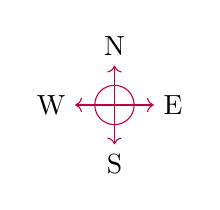
\begin{tikzpicture}[scale=0.5,draw=purple]
    \draw[<->] 
      (1,0) node[right] {E} 
      -- (-1,0) node[left] {W};
    \draw[<->]
      (0,1) node[above] {N} 
      -- (0,-1) node[below] {S};
    \draw (0,0) circle (0.5);

  \end{tikzpicture}


\end{questions}

\end{document}